\chapter{Background knowledge}
\label{sec:background}

Before attempting to answer our research questions, it is necessary to explain the relevant parts of Ask-Elle's architecture. This chapter presents the concepts of \emph{programming strategy}, \emph{program equivalence} and \emph{program unification}.

\section{Programming strategies}

As mentioned in Chapter \ref{sec:intro}, an exercise in Ask-Elle is a request to implement a function that matches one of the model solutions. Under the hood, Ask-Elle  generates a \emph{programming strategy} that specifies how an exercise can be solved, as a series of steps that go from an empty program to one of the model solutions.

Alternatively, we can think of a strategy as a finite-state machine. The initial state is the empty program, the transitions are the refinement steps and the accepting states are the model solutions.

Consider, for example, the model solution to the problem presented in Section \ref{sec:intro-askelle-example-session} (defined as \haskell{double = map (* 2)}). Figure \ref{fig:bg-fsm-prog-strategies} shows the generated strategy.

\begin{figure}
\centering
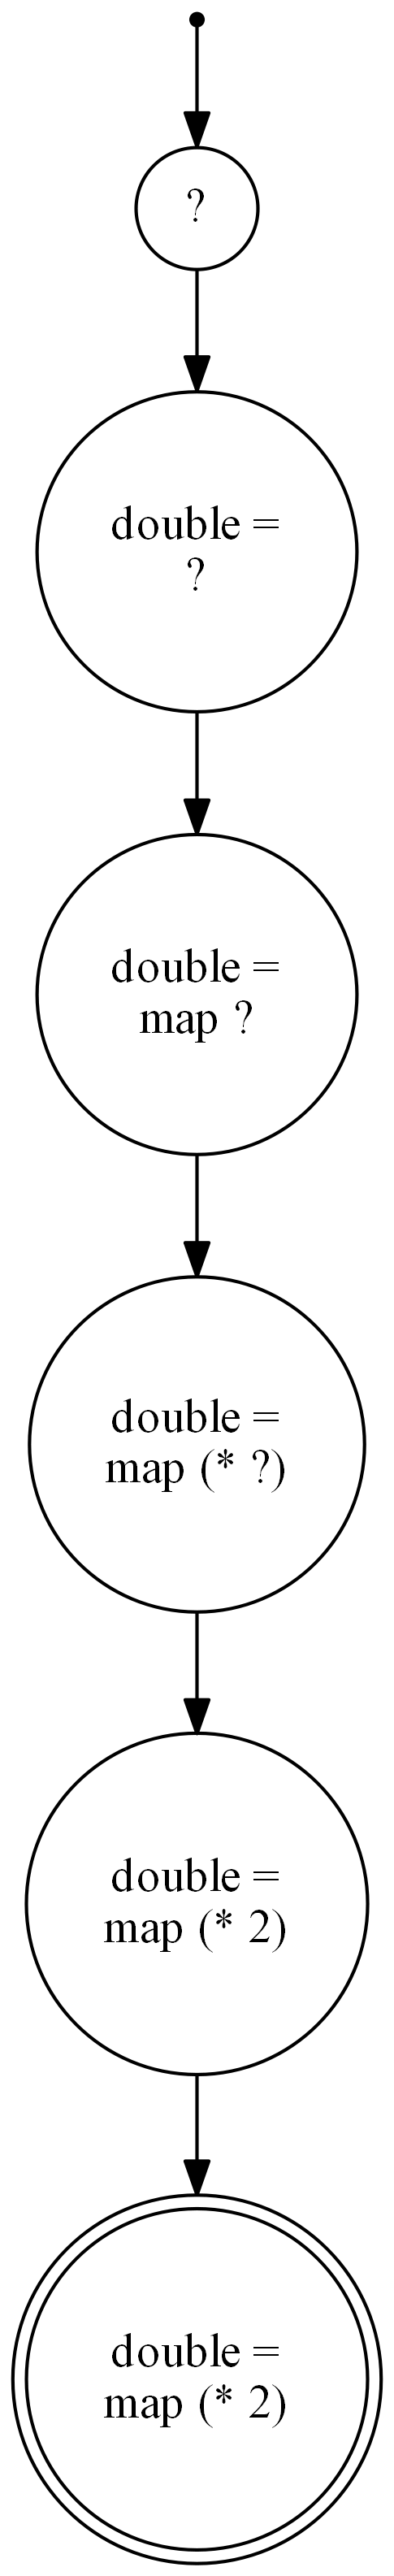
\includegraphics[height=20cm]{graphs/bg-fsm-prog-strategies}
\caption{Example of an Ask-Elle strategy}
\label{fig:bg-fsm-prog-strategies}
\end{figure}

According to the finite-state machine perspective on strategies, the algorithm used by Ask-Elle to provide hints works in two steps:

\begin{enumerate}
    \item Translate the student's program to a state in the machine;
    \item Retrieve a list of all transitions available from that state and present them in a user-friendly fashion.
\end{enumerate}

From these two steps, the second is a common operation on finite-state machines. The first one, however, is much more involved, as it requires unifying programs.

\section{Program equivalence}
\label{sec:bg-program-equivalence}

Before diving into the concept of program unification we need to refer to program equivalence, which comes in three flavors.

A basic form of program equivalence is \emph{syntactic equivalence}, according to which two programs are considered equivalent if their abstract syntax trees are equal. In its simplicity, this kind of equivalence has clear limitations. For instance, it does not account for differences in variable names or in the structure of the code.

More advanced is \emph{semantic equivalence}, according to which two programs are considered equivalent if their output is similar for all possible inputs. In the context of Ask-Elle, programs are functions, inputs are function parameters and the input domain consists of all possible values of the parameter types. In this case, differences in variable names are ignored, as well as differences in the structure of the code, as long as they have no influence in the output of the program. For Haskell, this also means that it does not take laziness into account, unless it has an impact on the output.

Finally, semantic equivalence \emph{up to preconditions} relaxes previous definition. Instead of requiring that two programs produce the same output for all possible inputs, this kind of equivalence considers only inputs that satisfy the preconditions of the program. Note that we assume the same preconditions to hold for both programs.

\section{Program unification}
\label{sec:bg-unification}

The process of comparing two programs for semantic equivalence up to holes is called program unification. This is what Ask-Elle does when comparing a student program to a model solution.

Since the problem of program unification is undecidable in the case of a complex language such as Haskell (see Section \ref{sec:related-work-unification}), Ask-Elle's unification procedure has the following possible outcomes:

\begin{enumerate}
    \item The programs are semantically equivalent;
    \item One program is an incomplete version of the other;
    \item Equivalence cannot be concluded.
\end{enumerate}

At the core of Ask-Elle's unification mechanism is the idea of normalization. Before comparing the programs, they go through a series of semantics-preserving transformations that result in a normal form. This way, comparing the programs becomes as simple as syntactically unifying the resulting normal forms.

Consider, for instance, the \texttt{double} function we mentioned before. Figure \ref{fig:bg-unification-normalization} shows a model solution, a possible student answer and the normalized version of both programs. This is an example of how a small syntactical difference, an unnecessary anonymous function, is ignored thanks to semantics-preserving transformations.

\begin{figure}[H]
\begin{minted}{haskell}
-- Model solution
double = map (* 2)

-- Student answer
double = map (\x -> 2 * x)

-- Normalized version (similar for both)
double = map ((*) 2)
\end{minted}
\caption{Example of unification by normalization}
\label{fig:bg-unification-normalization}
\end{figure}
